\documentclass{article}
\usepackage[utf8]{inputenc}
\usepackage{graphicx}
\usepackage[margin=1in]{geometry}
\usepackage[dvipsnames]{xcolor}
\usepackage{url}
\usepackage{hyperref}
\usepackage[numbers]{natbib} % for numeric references
\usepackage{amsmath}
\usepackage{booktabs}
\usepackage{float}
 
\begin{document}
 
\begin{titlepage}
    \begin{center}
        
\includegraphics[width=3cm]{image_msp.jpeg}
        \vspace{1cm}
        
        \textbf{\LARGE Global Distribution of Excess Nitrogen per Hectare of Cropland:}\\
        \textbf{\LARGE Analysis of Excess Nitrogen from 2009}
        
        \vspace{1.5cm}
        
        \textbf{\Large Hamza Ammi (ID6431492)}
        
        \vfill
        
        \large Date: \today
        
    \end{center}
\end{titlepage}
 
\newpage
 
\section*{Introduction}
Nitrogen is very important for the production of crops and food, but nitrogen that is not removed from the ground by harvested crops can remain in the environment. The data set used in this project measures the excess nitrogen per hectare of cropland, defined as the difference between nitrogen inputs (fertilizers, manure, fixation) and the nitrogen removed through harvested crops.
 
The research question is:
 
\begin{quote}
\textbf{How is excess nitrogen per hectare of cropland distributed across countries and continents in 2009? Is a positive nitrogen surplus common throughout the world, and what does the global distribution look like?}
\end{quote}
 
Each country or territory is treated as one observation, so percentages describe the observations and are not weighted by country area or population.
 
\section*{Data sample}
The dataset~\cite{owid_nitrogen} comes from Our World in Data and is based on research from West et al.~\cite{west2014}. The unit is kilograms of excess nitrogen per hectare of cropland (kg/ha).
 
In the data file there are 193 observations from the year 2009. There are no missing values. A continent column is added in the Python analysis to be able to draw conclusions on continent level.
 
The dataset was loaded with \texttt{pandas.read\_csv}. The nitrogen measurements were converted to a NumPy array to do statistical analysis. The mean, median, standard deviation, minimum, and maximum were calculated. The uncertainty of the mean is represented by the standard error,
\[
SE = \frac{s}{\sqrt{n}},
\]
where $s$ is the sample standard deviation and $n$ is the number of observations.
 
The distribution was examined with a histogram and by calculating the skewness and excess kurtosis. The proportion of positive observations was calculated, and a simple binomial-style uncertainty is used for this proportion:
\[
SE_p = \sqrt{\frac{p(1-p)}{n}}.
\]
The same mean, median, standard deviation and positive-surplus percentage calculations were repeated for each continent.
 
\section*{Results and discussion}
For all 193 observations, the mean excess nitrogen was 42.50 kg/ha, with a standard error of 5.14 kg/ha. The median was 27.63 kg/ha and the standard deviation was 71.35 kg/ha. The minimum was -210.01 kg/ha and the maximum was 313.79 kg/ha.
 
A positive surplus occurred in 154 of 193 observations, or 79.8\%. The binomial-style standard uncertainty of this percentage is approximately 2.9 percentage points. Thus, positive excess nitrogen is present in most of the observations in this dataset, however this cannot be interpreted as a percentage of global cropland.
 
\begin{table}[H]
\centering
\small
\begin{tabular}{lrrrr}
\toprule
Continent & $N$ & Mean & Median & Positive (\%)\\
\midrule
Africa & 53 & 16.41 & 11.57 & 79.25\\
Asia & 51 & 81.76 & 61.63 & 86.27\\
Europe & 39 & 58.14 & 49.72 & 97.44\\
North America & 30 & 18.25 & 13.17 & 53.33\\
South America & 13 & 47.44 & 57.07 & 92.31\\
Oceania & 7 & -38.44 & -56.12 & 28.57\\
\bottomrule
\end{tabular}
\caption{Simple continent-level summary. Means and medians are in kg/ha.}
\end{table}
 
\begin{figure}[H]
\centering
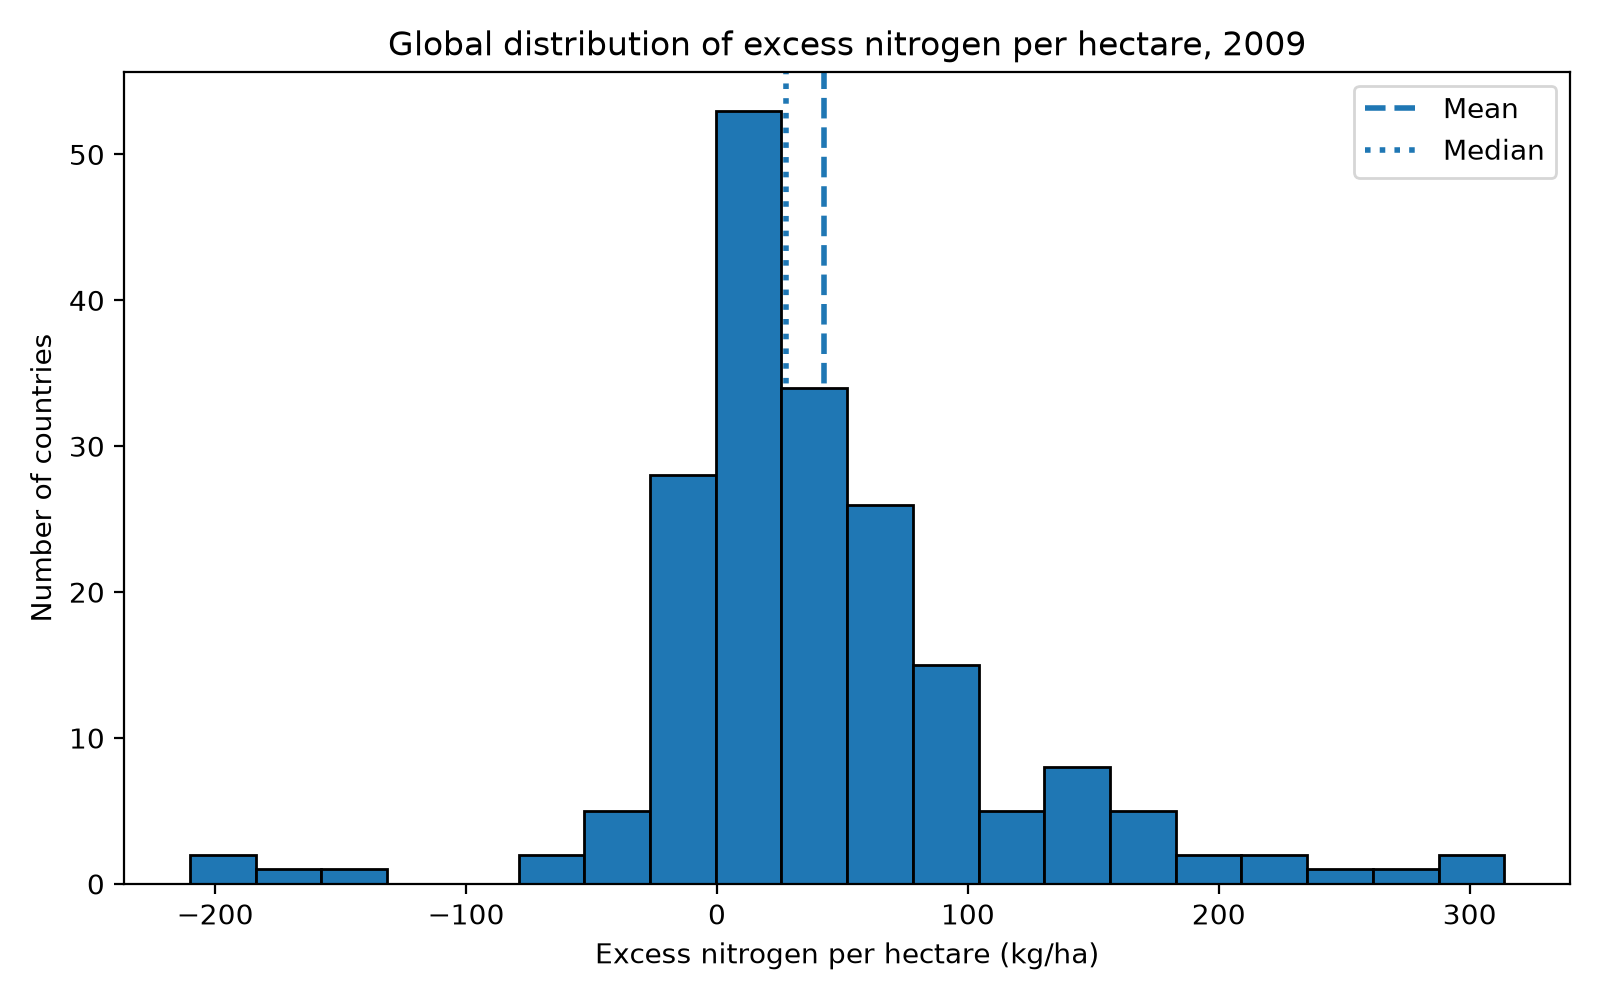
\includegraphics[width=0.78\textwidth]{global_distribution.png}
\caption{Distribution of excess nitrogen per hectare across the 193 observations. The dashed line is the mean and the dotted line is the median.}
\end{figure}
 
The global histogram is not well described by a normal distribution. The mean (42.50 kg/ha) is higher than the median (27.63 kg/ha), and the skewness is 0.60. The excess kurtosis is 3.50, indicating heavy tails compared with a normal distribution. This is consistent with several very high positive and very low negative observations.
 
\subsection*{Conclusion}
The analysis shows that the dataset has a broad global distribution of excess nitrogen per hectare. A positive surplus occurs in 79.8\% of the 193 observations. However, the standard deviation is 71.35 kg/ha, compared with a mean of 42.50 kg/ha, and the minimum and maximum are far from zero. The continent-level means also differ, with the largest mean in Asia (81.76 kg/ha) and a negative mean in Oceania ($-$38.44 kg/ha).
 
These results describe the distribution of country/territory observations. They do not measure the percentage of global cropland with a surplus, because the observations are not weighted by cropland area. The dataset also contains only the year 2009.
 
\begin{thebibliography}{9}
 
\bibitem{owid_nitrogen}
Our World in Data. 
\textit{Excess nitrogen per hectare of cropland}. 
Available at: \href{https://ourworldindata.org/grapher/excess-nitrogen-per-hectare}{https://ourworldindata.org/grapher/excess-nitrogen-per-hectare}.
 
\bibitem{west2014}
West, P. C., et al. (2014). 
Leverage points for improving global food security and the environment. 
\textit{Science}, 345(6194), 325--328.
 
\end{thebibliography}
\end{document}
 
